\nameref{sub:array}s offer a means of storing and working with a list of values in your code. Each array has a number of elements, each of which has a value, and can be accessed using an index. Together with the \nameref{sub:for_loop}, arrays provide a means of managing multiple values in your code. The following illustrations show how these work in the computer, and should help you better understand how arrays can be used within your code.

\subsection{Understanding Populate Array} % (fold)
\label{sub:understanding_populate_array}

\sref{sub:designing_statistics_calculator} \nameref{sub:designing_statistics_calculator} outlined the pseudocode and flowcharts for a small statistics programs. This included a number of functions and procedures that helped divide the Program's code into smaller units of work. One of these procedures was \texttt{Populate Array}, discussed in \sref{ssub:populating_the_array} \nameref{ssub:populating_the_array}. This procedure is responsible for reading values from the user and using these to populate the program's array, and the flowchart for this logic is shown in \fref{fig:populate-array-flow-understanding}.

\begin{figure}[htbp]
   \centering
   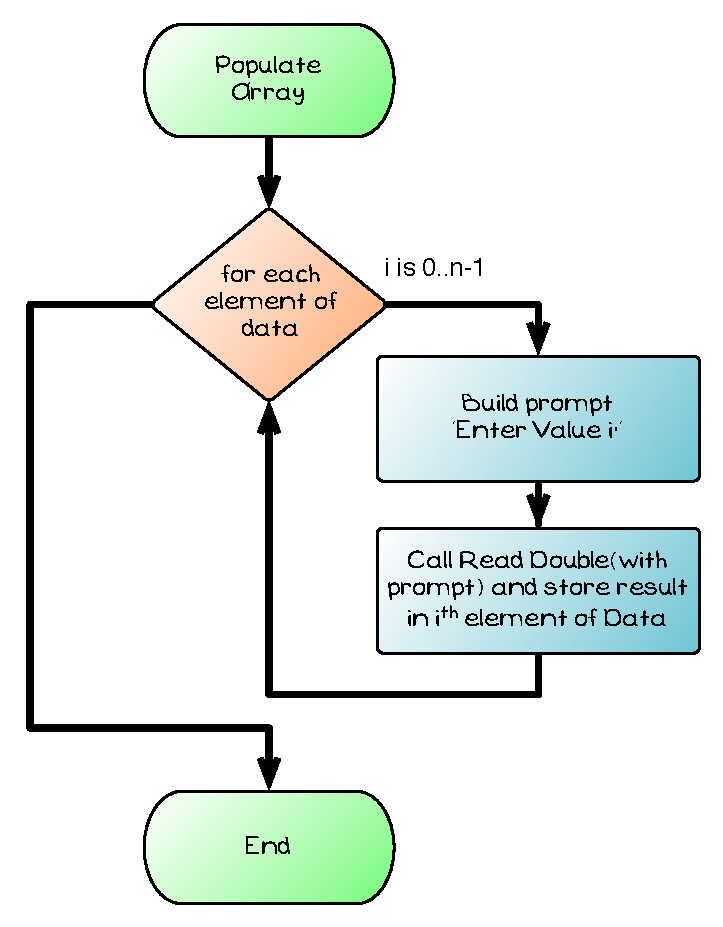
\includegraphics[width=0.5\textwidth]{./topics/arrays/diagrams/PopulateArray} 
   \caption{Flowchart showing the process for \texttt{Populate Array}, from \fref{fig:populate-array-flow}}
   \label{fig:populate-array-flow-understanding}
\end{figure}

The following illustrations will show this code running to populate an array that contains three values. This will show how the array is passed by reference, and how the for loop works together with the array to populate all elements.

\clearpage
\subsubsection{Main starts, and the array is allocated space} % (fold)
\label{ssub:main_starts_and_the_array_is_allocated_space}

All local variables are allocated space on the Stack when the function or procedure they are declared in is called. In this example the \texttt{Main} procedure is executed and space is allocated for its \texttt{my\_data} variable. This variable is an \nameref{sub:array} that is used to store three \texttt{double} values. When \texttt{Main} is loaded onto the Stack there is space allocated for three \texttt{double} values associated with the \texttt{my\_data} variable.

\begin{figure}[htbp]
   \centering
   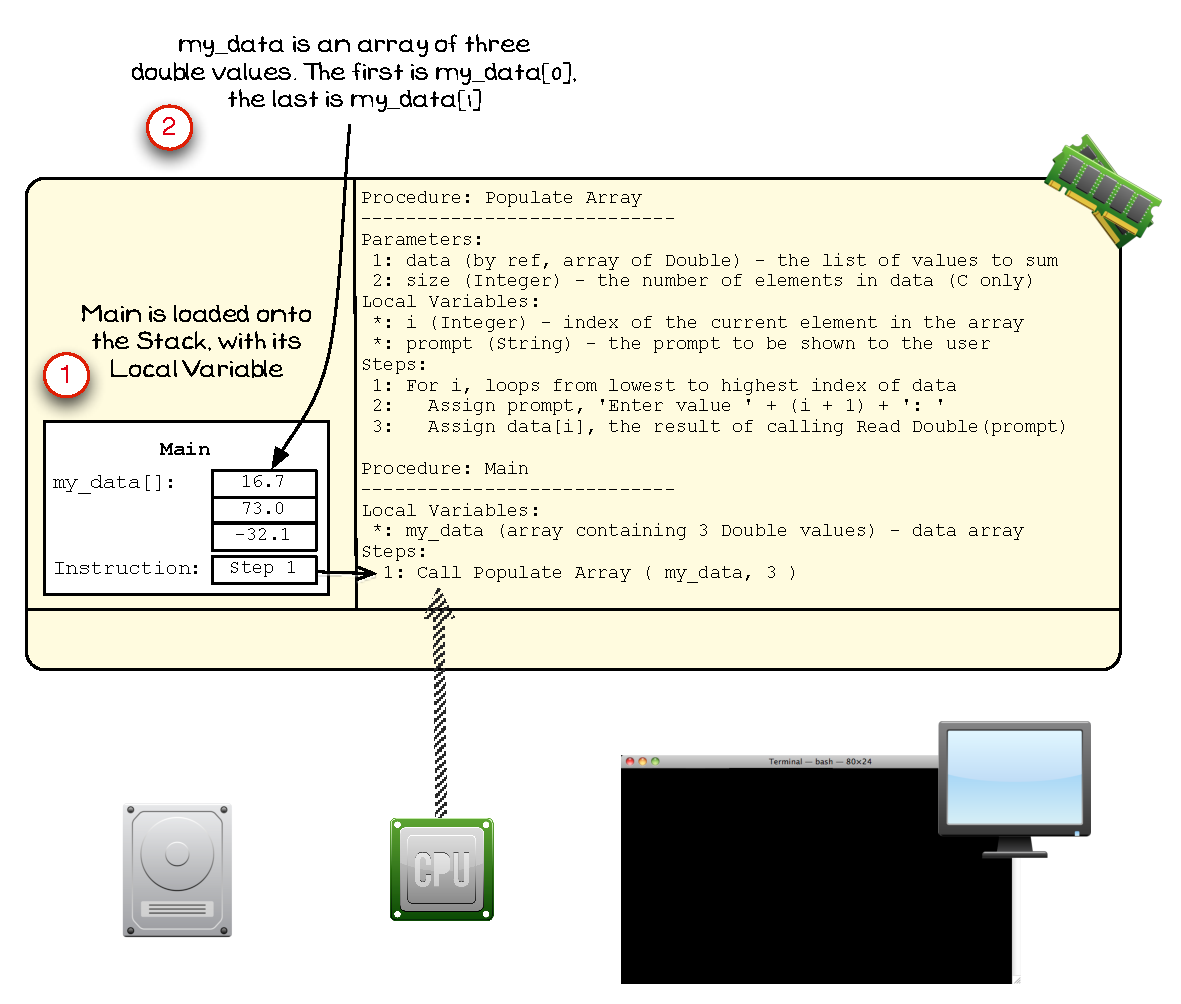
\includegraphics[width=\textwidth]{./topics/arrays/images/PopulateArray1} 
   \caption{When the program starts \texttt{Main} allocates space for its local variables, including the array}
   \label{fig:populate-array-vis-1}
\end{figure}

\mynote{
\begin{itemize}
  \item In \fref{fig:populate-array-vis-1} the indicated areas show the following:
  \begin{enumerate}
    \item The Program starts and \texttt{Main} is loaded onto the stack, allocating space for its local variables.
    \item The \texttt{my\_data} array is allocated space to store its values.
  \end{enumerate}
  \medskip
  \item Notice that the three values in the array are allocated next to each other.
  \item The indexes can be used to access the array's elements. The index value determines the number of elements that must be skipped to find where the value is stored.
\end{itemize}
}
% subsubsection main_starts_and_the_array_is_allocated_space (end)

\clearpage
\subsubsection{Populate array is called, and a reference to \texttt{my{\textunderscore}data} passed in} % (fold)
\label{ssub:populate_array_is_called_and_a_reference_to_my_data_passed_in}

\texttt{Populate Array} is called as the first step in \texttt{Main}. This is passed the \texttt{my\_data} variable (pass by reference), rather than being passed the values from within that variable. This gives the \texttt{data} parameter access to the memory where \texttt{my\_data} is stored.

\begin{figure}[htbp]
   \centering
   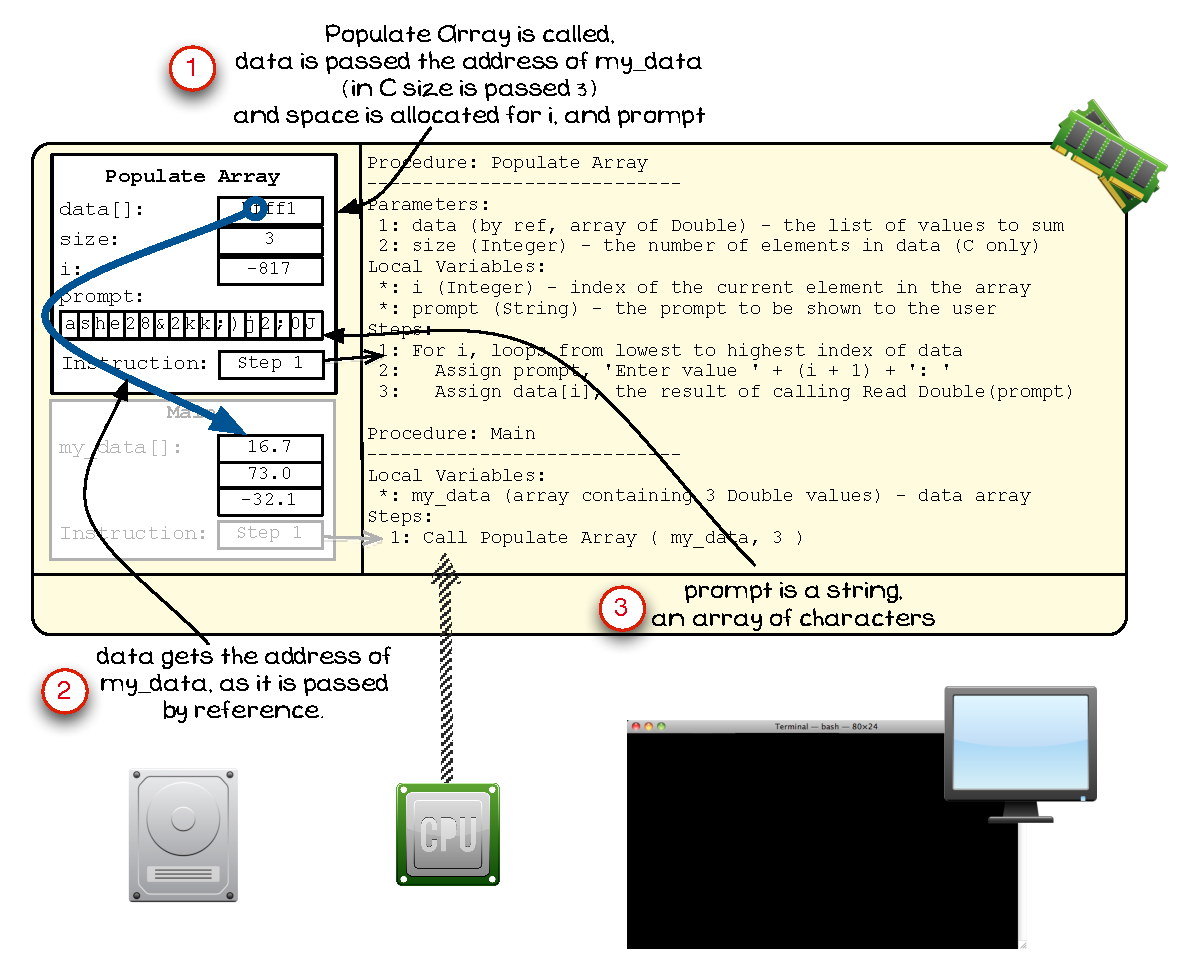
\includegraphics[width=\textwidth]{./topics/arrays/images/PopulateArray2} 
   \caption{Populate array is called, and a reference to the \texttt{my\_data} array is pass to its \texttt{data} parameter}
   \label{fig:populate-array-vis-2}
\end{figure}

\mynote{
\begin{itemize}
  \item In \fref{fig:populate-array-vis-2} the indicated areas show the following:
  \begin{enumerate}
    \item When \texttt{Populate Array} is called it is loaded onto the Stack. Its \texttt{data} parameter receives the address of \texttt{my\_data} from \texttt{Main}. In C the value 3 would also be passed to the \texttt{size} parameter, as C does not keep track of the length of the array for you. At the same time space for \texttt{Populate Array}'s local variables \texttt{i} and \texttt{prompt} are allocated on the Stack.
    \item Notice that in \texttt{Populate Array} the \texttt{data} parameter only stores the address of the array, as it is passed by reference. This saves time and space, and is needed in this case as the procedure wants to store data into the variable passed to this parameter.
    \item The \texttt{prompt} local variable is also an array. It is allocated spaces on the stack as is done for all local variables. 
  \end{enumerate}
  \medskip
  \item Arrays are allocated a contiguous area of memory to store its elements.
  \item A String is an array of characters.
\end{itemize}
}

% subsubsection populate_array_is_called_and_a_reference_to_my\_data_passed_in (end)

\clearpage
\subsubsection{Step 1 of \texttt{Populate Array} is run} % (fold)
\label{ssub:step_1_of_populate_array_is_run}

Step 1 of \texttt{Populate Array} initialises the for loop's control variable (\texttt{i} in this case). This variable keeps track of the times the loop body has executed, and can be used to get the \emph{current} value from the array.

\begin{figure}[htbp]
   \centering
   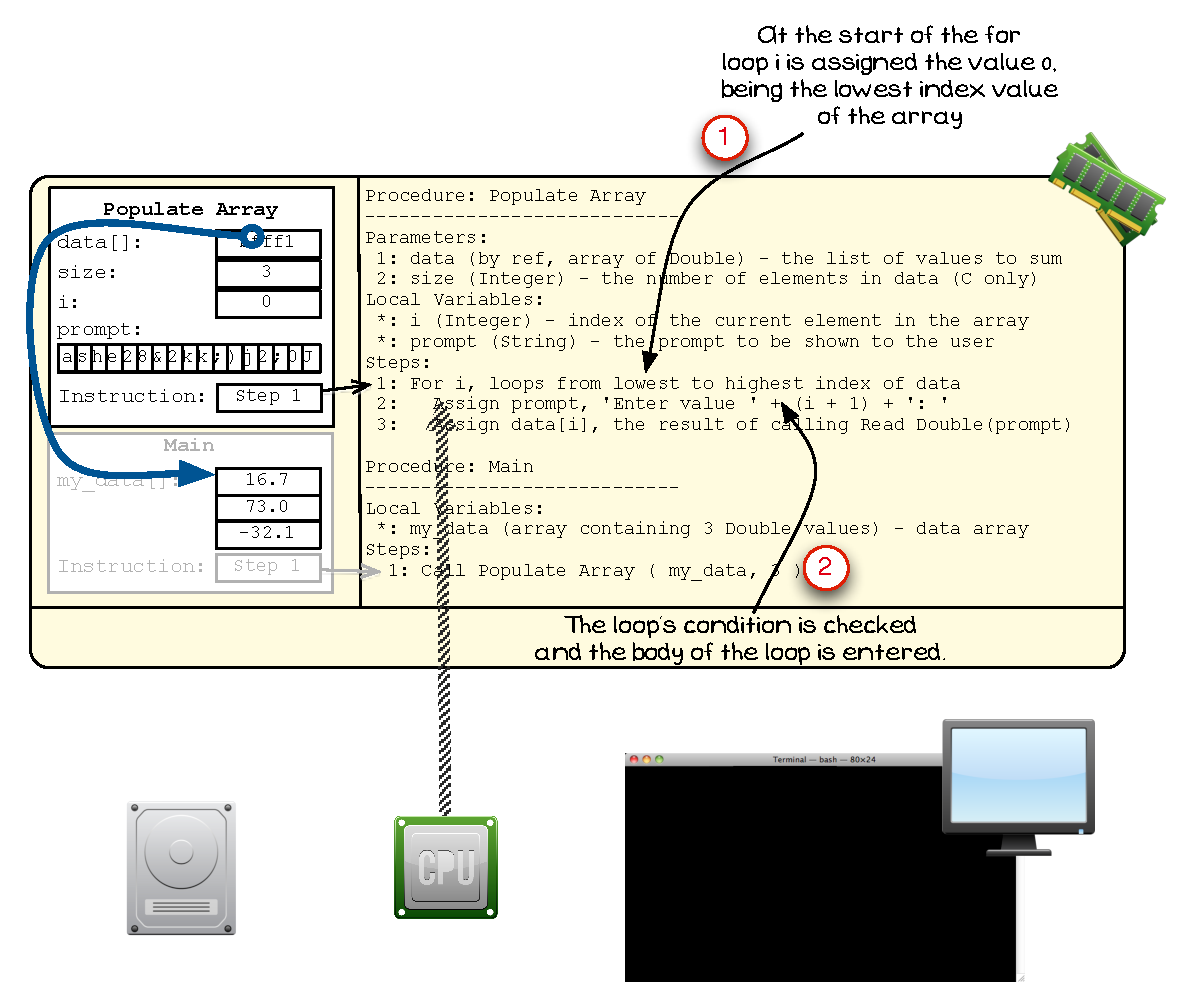
\includegraphics[width=\textwidth]{./topics/arrays/images/PopulateArray3} 
   \caption{Step 1 of \texttt{Populate Array} is called, and the for loop sets i to the lowest index of the \texttt{data} array}
   \label{fig:populate-array-vis-3}
\end{figure}

\mynote{
\begin{itemize}
  \item In \fref{fig:populate-array-vis-3} the indicated areas show the following:
  \begin{enumerate}
    \item Step 1 of \texttt{Populate Array} is a for loop. The first action of the for loop is to initialise the value of \texttt{i} to the \emph{lowest index value} of the \texttt{data} array. The lowest index is 0, so \texttt{i} is assigned the value 0.
    \item Next the loop checks its condition, it is loop from 0 to 2, and has not passed 2 so the body of the loop will be executed. This will be checked again when the for loop ends.
  \end{enumerate}
  \medskip
  \item The first action of a for loop is to initialise the value of the control variable.
  \item When processing each element of an array the for loop should initialise the control variable to 0, the first index of the array.
\end{itemize}
}

% subsubsection step_1_of_populate_array_is_run (end)

\clearpage
\subsubsection{Step 2 constructs the prompt to be shown to the user} % (fold)
\label{ssub:step_2_constructs_the_prompt_to_be_shown_to_the_user}

The user needs to be told what to enter. The \texttt{prompt} is a string that will contain this message so that it can be passed to \texttt{Read Double}. The value for the prompt will use the loop's control variable (the counter) so that the user known which value they are up to.

\begin{figure}[htbp]
   \centering
   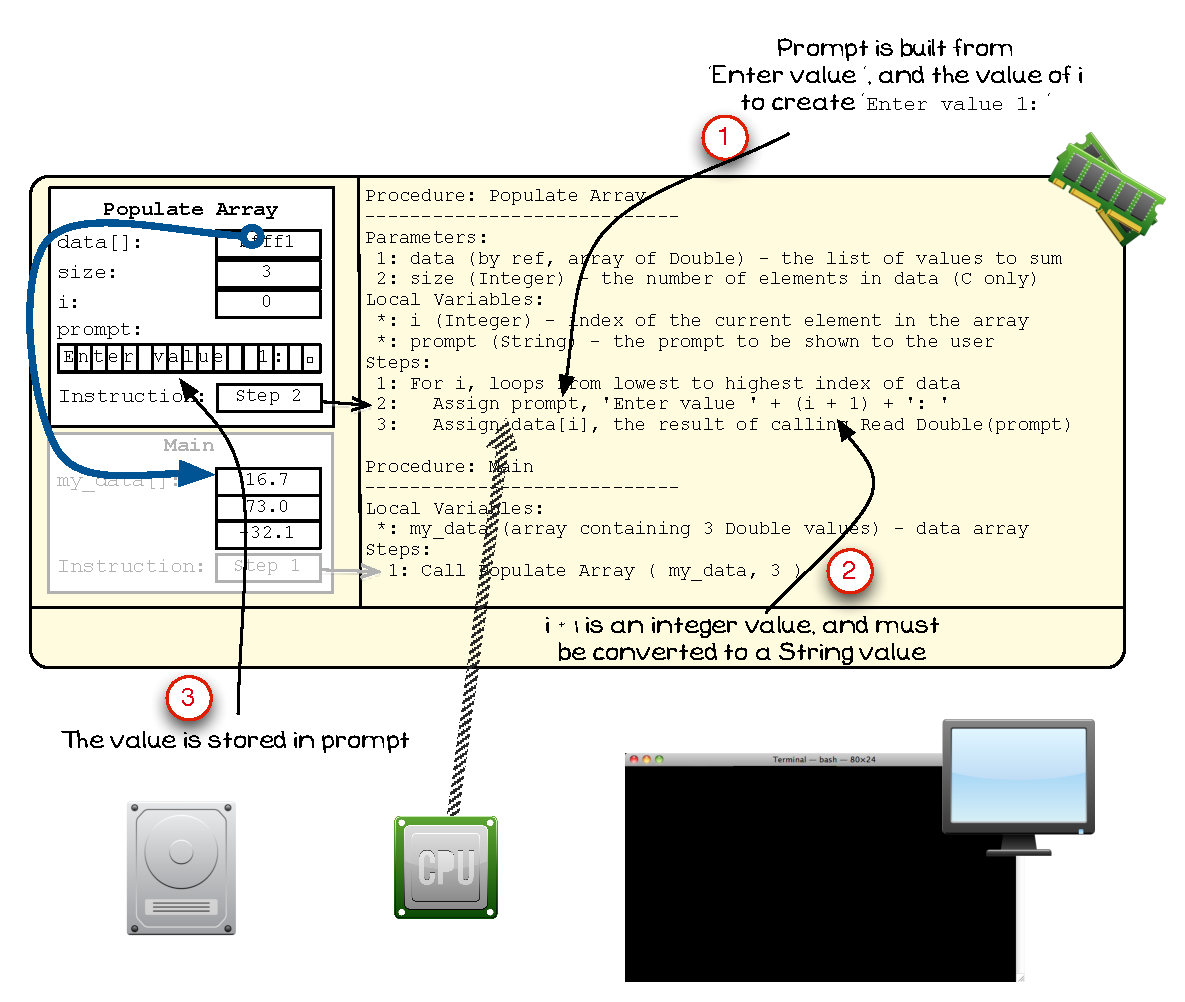
\includegraphics[width=\textwidth]{./topics/arrays/images/PopulateArray4} 
   \caption{Step 2 builds the prompt \texttt{Enter value 1: } which will be shown to the user}
   \label{fig:populate-array-vis-4}
\end{figure}

\mynote{
\begin{itemize}
  \item In \fref{fig:populate-array-vis-4} the indicated areas show the following:
  \begin{enumerate}
    \item Step 2 of \texttt{Populate Array} builds the prompt by concatenating `\texttt{Enter Value}' with \texttt{i + 1} and `\texttt{: }'.
    \item To achieve this \texttt{i + 1} must be converted from an Integer to a String.
    \item The result is stored in the \texttt{prompt} variable.
  \end{enumerate}
  \medskip
  \item This action will be performed each time the loop executes. In this case the value stored in \texttt{prompt} will be `\texttt{Enter value  1: }'.
  \item The small square shown at the end of the \texttt{prompt} represents the overhead. In C this is the \emph{sentinel} value, in Pascal it is the length\footnote{Pascal actually stores the length at the start of the string, but the idea is the same.} of the array.
\end{itemize}
}


% subsubsection step_2_constructs_the_prompt_to_be_shown_to_the_user (end)

\clearpage
\subsubsection{Step 3 reads a value from the user and stores it in the array at index 0} % (fold)
\label{ssub:step_3_reads_a_value_from_the_user_and_stores_it_in_the_array_at_index_0}

The next step calls the \texttt{Read Double} function. This is responsible for reading a value from the user, and returning it to the caller. The value returned is then stored in an element of the array. The \texttt{i} variable is read to determine the position where this value should be stored. This means that you can think of \texttt{i} as referring to the \emph{current} element of the array.

\begin{figure}[htbp]
   \centering
   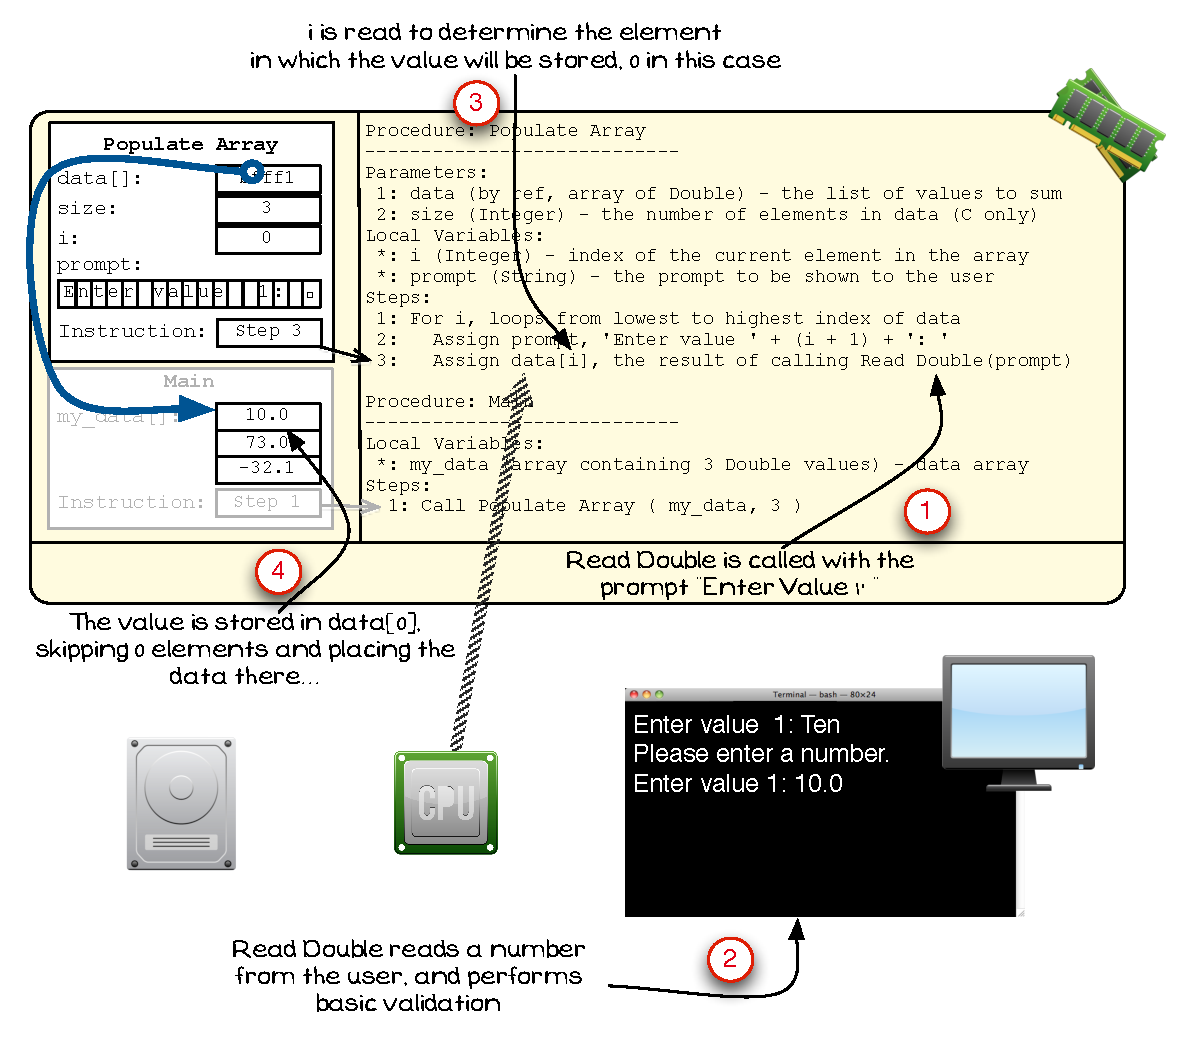
\includegraphics[width=\textwidth]{./topics/arrays/images/PopulateArray5} 
   \caption{Step 3 reads a \texttt{double} value from the user and stores it in \texttt{data[i]}}
   \label{fig:populate-array-vis-5}
\end{figure}

\mynote{
\begin{itemize}
  \item In \fref{fig:populate-array-vis-5} the indicated areas show the following:
  \begin{enumerate}
    \item Step 3 of \texttt{Populate Array} calls \texttt{Read Double}, passing across the prompt to be shown to the user.
    \item Within \texttt{Read Double} the value is read from the Terminal. This includes some validation to make sure that the value entered is a number.
    \item To determine where the value is stored the computer needs to evaluate the expression used to index the array. In this case that is the value of the \texttt{i} variable.
    \item The \texttt{data} reference is followed, and \texttt{0} elements skipped, to find the location where the data should be stored. 
  \end{enumerate}
  \medskip
  \item Notice that this has stored the value in \texttt{my\_data}, as \texttt{data} is passed by reference.
\end{itemize}
}

% subsubsection step_3_reads_a_value_from_the_user_and_stores_it_in_the_array_at_index_0 (end)

\clearpage
\subsubsection{Control returns to Step 1 as the loop body has ended} % (fold)
\label{ssub:control_returns_to_step_1_as_the_loop_body_has_ended}

At the end of the loop body the for loop performs two actions. It has finished the first pass through the loop, so its control variable (the counter) needs to be incremented to 1. Then it needs to jump back to check its condition. This will determine if the loop's body is executed again or skipped. In this case \texttt{i} is still in the defined range so the loop's body is run again.

\begin{figure}[htbp]
   \centering
   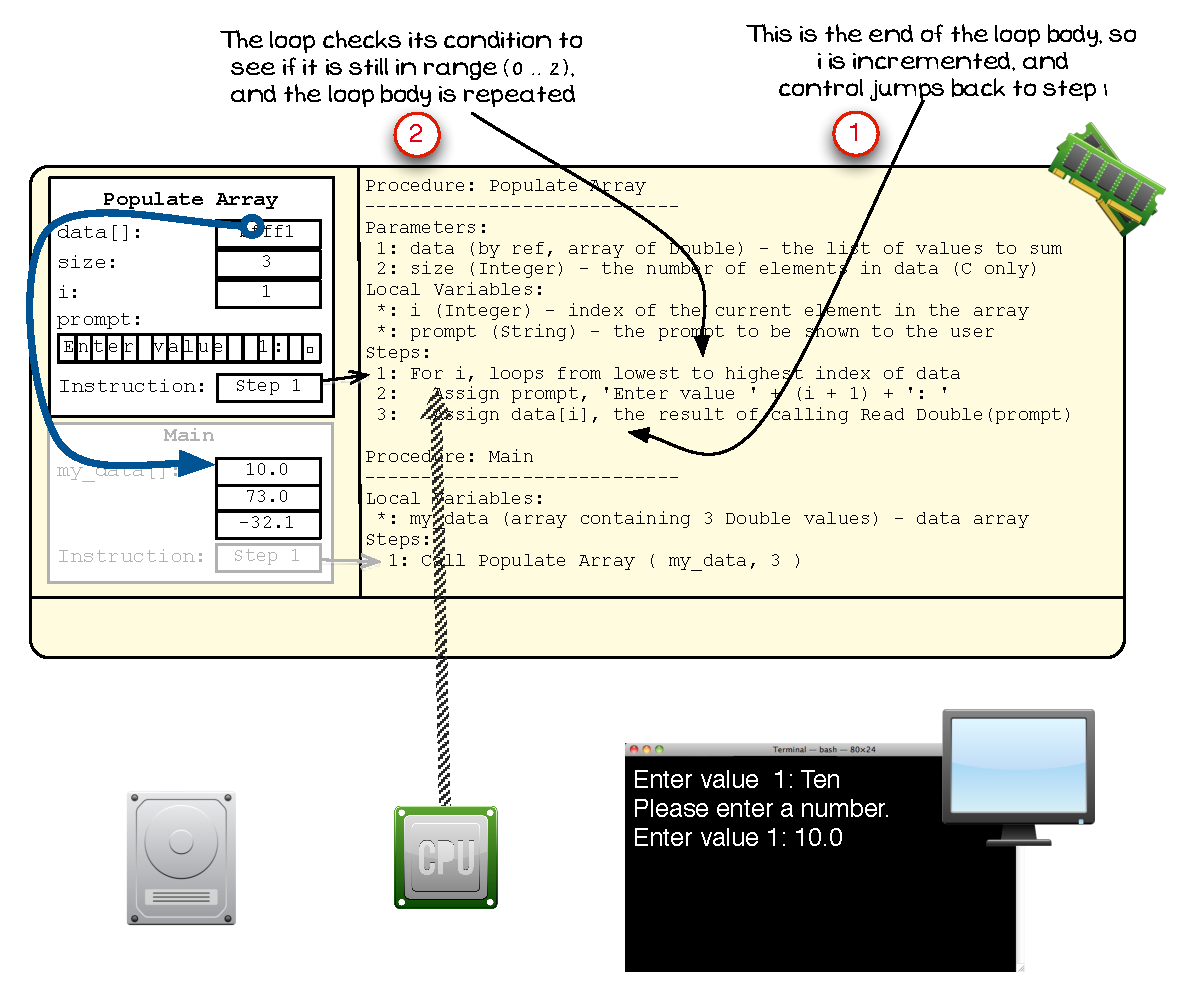
\includegraphics[width=\textwidth]{./topics/arrays/images/PopulateArray6} 
   \caption{At the end of the loop body \emph{i} is incremented and control jumps back to check the loop's condition}
   \label{fig:populate-array-vis-6}
\end{figure}

\mynote{
\begin{itemize}
  \item In \fref{fig:populate-array-vis-6} the indicated areas show the following:
  \begin{enumerate}
    \item The end of the loop body indicates that two things needs to occur. Firstly the value of \texttt{i} needs to be incremented, and then control needs to jump back to check the condition of the loop (step 1).
    \item The loop's condition checks if \texttt{i} is still in range (\texttt{i} is in the range \texttt{0..2}, coded as \texttt{i < size} in C). As it is still in range the loop's body will execute again.
  \end{enumerate}
  \medskip
\end{itemize}
}

% subsubsection control_returns_to_step_1_as_the_loop_body_has_ended (end)

\clearpage
\subsubsection{Second prompt is built, asking the user to enter value 2} % (fold)
\label{ssub:second_prompt_is_built_asking_the_user_to_enter_value_2}

Back at step 2 again, the prompt needs to be recreated. This time its message will be `\texttt{Enter value 2: }'. The process to create this is the same, with the value of \texttt{i + 1} being converted to a String, and the three parts concatenated together and stored in \texttt{prompt}. This overrides the details in the existing array, reusing the same memory to store these values.

\begin{figure}[htbp]
   \centering
   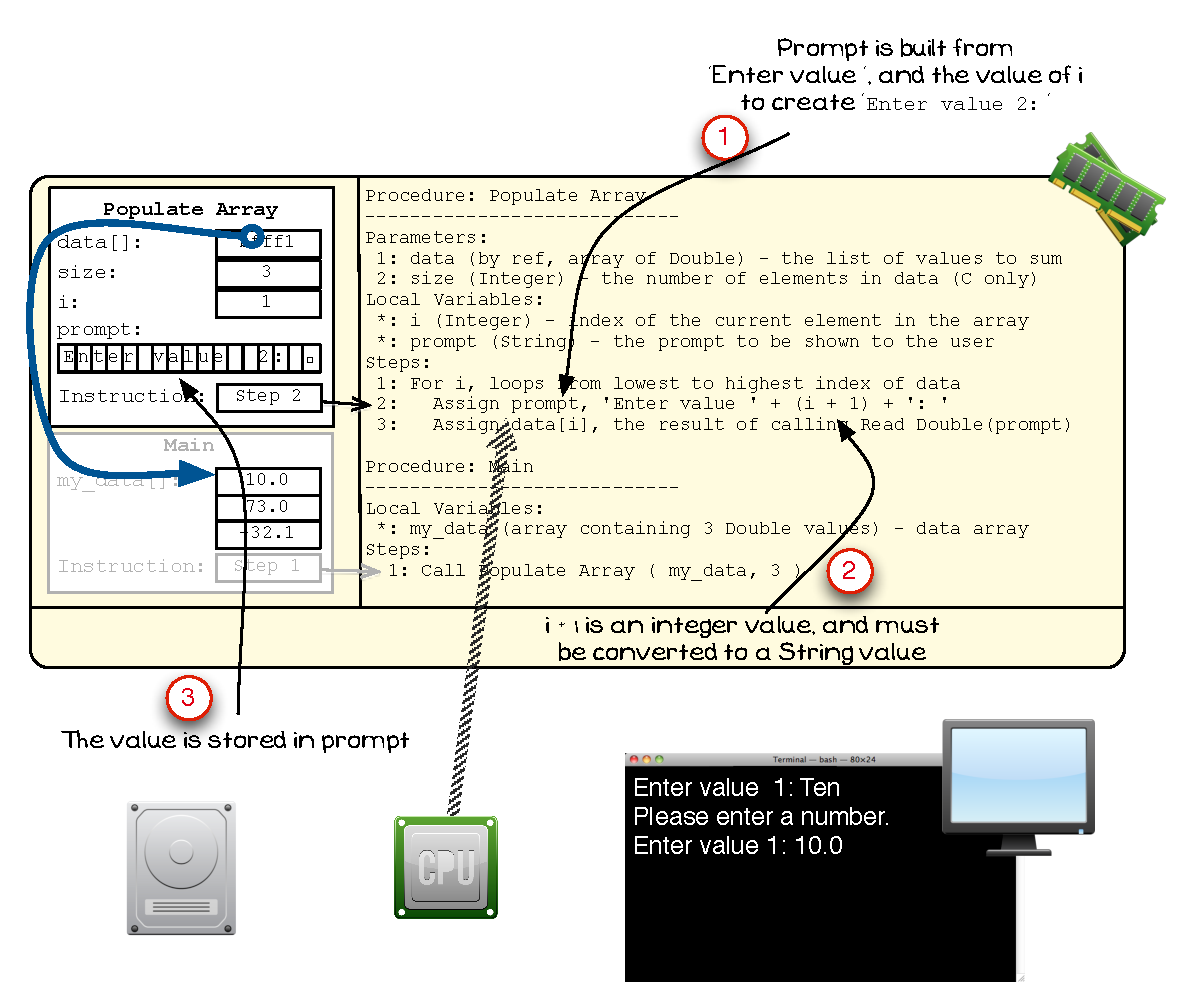
\includegraphics[width=\textwidth]{./topics/arrays/images/PopulateArray7} 
   \caption{Step 2 builds the prompt \texttt{Enter value 2: } which will be shown to the user}
   \label{fig:populate-array-vis-7}
\end{figure}

\mynote{
\begin{itemize}
  \item In \fref{fig:populate-array-vis-7} the indicated areas show the following:
  \begin{enumerate}
    \item Step 2 of \texttt{Populate Array} builds the prompt by concatenating `\texttt{Enter Value}' with \texttt{i + 1} and `\texttt{: }'.
    \item To achieve this \texttt{i + 1} must be converted from an Integer to a String.
    \item The result is stored in the \texttt{prompt} variable.
  \end{enumerate}
  \medskip
  \item Notice that this is using the same location to store its data.
  \item The small square shown at the end of the \texttt{prompt} represents the overhead. In C this is the \emph{sentinel} value, in Pascal it is the length\footnote{Pascal actually stores the length at the start of the string, but the idea is the same.} of the array.
\end{itemize}
}

% subsubsection second_prompt_is_built_asking_the_user_to_enter_value_2 (end)

\clearpage
\subsubsection{Populate Array stores the second value read into \texttt{data[1]}} % (fold)
\label{ssub:populate_array_stores_the_second_value_read_into_data[1]}

Step 3 uses \texttt{Read Double} again to get the value to store in the second element of the array. To find where this should be stored the computer calculates the value of the index, reading this from the \texttt{i} variable. The value returned from \texttt{Read Double} is then stored in the array referred to by \texttt{data}, at index \texttt{1}.

\begin{figure}[htbp]
   \centering
   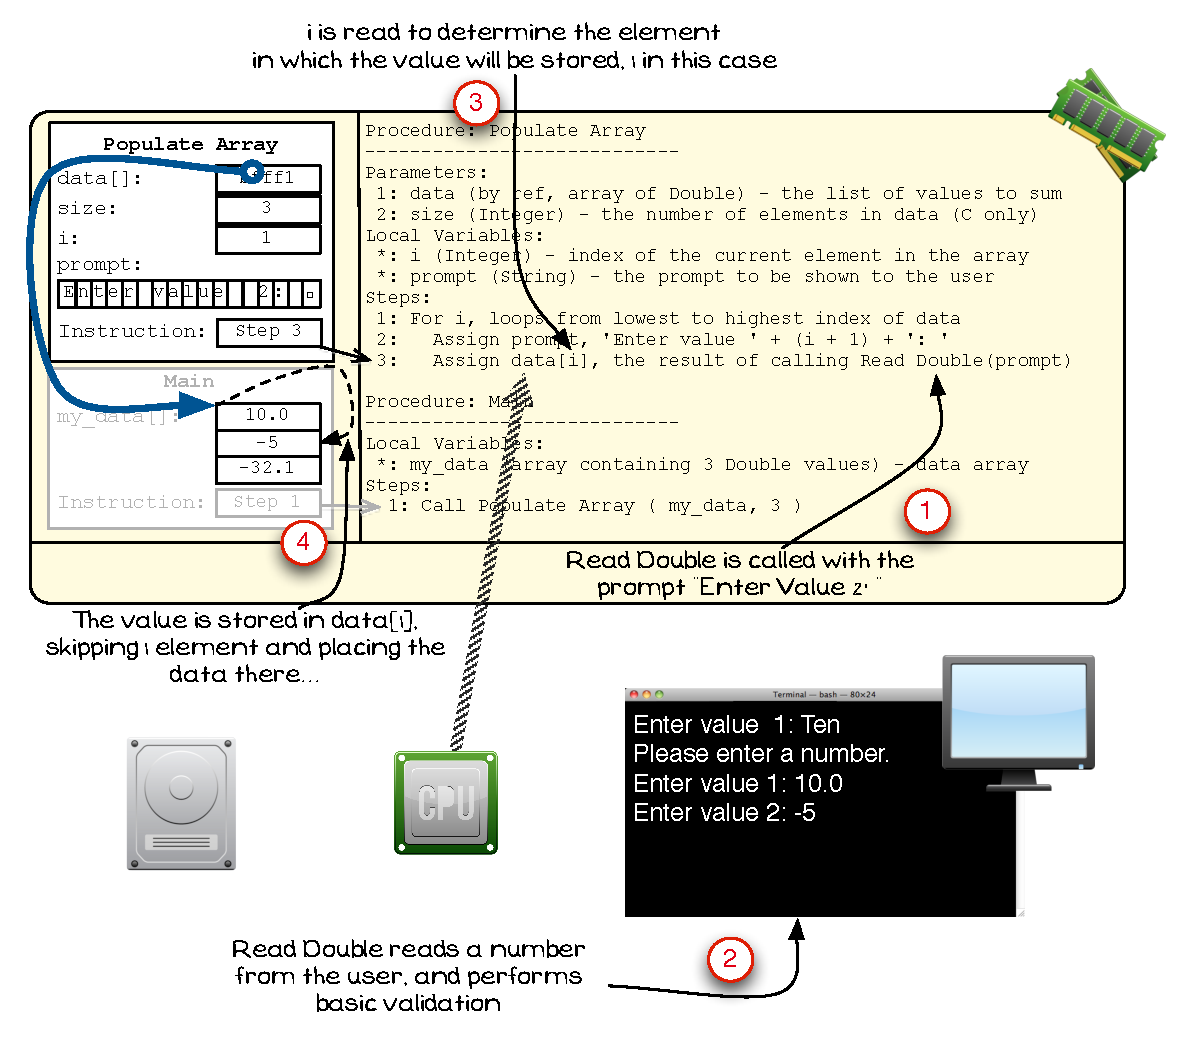
\includegraphics[width=\textwidth]{./topics/arrays/images/PopulateArray8} 
   \caption{The second value read is stored in \texttt{data[1]}}
   \label{fig:populate-array-vis-8}
\end{figure}

\mynote{
\begin{itemize}
  \item In \fref{fig:populate-array-vis-8} the indicated areas show the following:
  \begin{enumerate}
    \item Step 3 of \texttt{Populate Array} calls \texttt{Read Double}, passing across the prompt to be shown to the user.
    \item Within \texttt{Read Double} the value is read from the Terminal. This includes some validation to make sure that the value entered is a number.
    \item The value of the index is now \texttt{1}, as read from variable \texttt{i}.
    \item The \texttt{data} reference is followed, and \texttt{1} element is skipped, to find the location where the data should be stored.
  \end{enumerate}
  \medskip
\end{itemize}
}

% subsubsection populate_array_stores_the_second_value_read_into_data[1] (end)

% subsection understanding_populate_array (end) 